\documentclass{chi-ext}
% Please be sure that you have the dependencies (i.e., additional LaTeX packages) to compile this example.
% See http://personales.upv.es/luileito/chiext/

%% EXAMPLE BEGIN -- HOW TO OVERRIDE THE DEFAULT COPYRIGHT STRIP -- (July 22, 2013 - Paul Baumann)
% \copyrightinfo{Permission to make digital or hard copies of all or part of this work for personal or classroom use is granted without fee provided that copies are not made or distributed for profit or commercial advantage and that copies bear this notice and the full citation on the first page. Copyrights for components of this work owned by others than ACM must be honored. Abstracting with credit is permitted. To copy otherwise, or republish, to post on servers or to redistribute to lists, requires prior specific permission and/or a fee. Request permissions from permissions@acm.org. \\
% {\emph{CHI'14}}, April 26--May 1, 2014, Toronto, Canada. \\
% Copyright \copyright~2014 ACM ISBN/14/04...\$15.00. \\
% DOI string from ACM form confirmation}
%% EXAMPLE END -- HOW TO OVERRIDE THE DEFAULT COPYRIGHT STRIP -- (July 22, 2013 - Paul Baumann)

\title{QuizCram: A Question-Driven Video Studying Interface}

\numberofauthors{1}
% Notice how author names are alternately typesetted to appear ordered in 2-column format;
% i.e., the first 4 autors on the first column and the other 4 auhors on the second column.
% Actually, it's up to you to strictly adhere to this author notation.
\author{
  \alignauthor{
  	\textbf{Geza Kovacs}\\
  	\affaddr{Department of Computer Science, Stanford University}\\
  	\email{geza@cs.stanford.edu}
  }
}

% Paper metadata (use plain text, for PDF inclusion and later re-using, if desired)
\def\plaintitle{QuizCram: A Question-Driven Video Studying Interface}
\def\plainauthor{Geza Kovacs}
\def\plainkeywords{video flashcards, lecture reviewing, in-video questions}
\def\plaingeneralterms{video flashcards, lecture reviewing, in-video questions}

\hypersetup{
  % Your metadata go here
  pdftitle={\plaintitle},
  pdfauthor={\plainauthor},  
  pdfkeywords={\plainkeywords},
  pdfsubject={\plaingeneralterms},
  % Quick access to color overriding:
  %citecolor=black,
  %linkcolor=black,
  %menucolor=black,
  %urlcolor=black,
}

\usepackage{graphicx}   % for EPS use the graphics package instead
\usepackage{balance}    % useful for balancing the last columns
\usepackage{bibspacing} % save vertical space in references

\usepackage[absolute]{textpos}

\usepackage{paralist}

\begin{document}

\maketitle

\begin{textblock}{5}(3.6,7.7)
\begin{figure}
\includegraphics[width=\columnwidth]{singlevideo-overview}
\caption{The QuizCram interface, showing the current video. The focus question is on left, and the associated video is on the right. The progressbar highlights the relevant portion of the video, and shows which segments have already been seen.}
\label{fig:figure1}
\end{figure}
\end{textblock}

\begin{abstract}
% Need some motivation here before jumping right into what we built
QuizCram is a question-focused format for navigating and reviewing lecture videos.
QuizCram shows users a question to answer, with an associated video segment.
Users navigate through the video segments by answering questions.
We also allow users to review using a timeline of previously answered questions and videos.
To encourage users to review questions, QuizCram keeps track of their question-answering and video-watching history and recommends users to review questions they have not fully mastered.
QuizCram-format courses can be generated automatically from lectures with in-video quizzes,
though the format is flexible enough to accommodate multiple questions per video segment.
Our user study comparing QuizCram to in-video quizzes finds that users
practice answering and reviewing questions more when using QuizCram, and
are better able to remember answers to questions they encountered.
\end{abstract}

\keywords{\plainkeywords}
%\textcolor{red}{Optional section to be included in your final version.}

\category{H.5.2.}{Information Interfaces and Presentation (e.g. HCI)}{Graphical User Interfaces}
%See \cite{ACMCCS} 
%See: \url{http://www.acm.org/about/class/1998/} 
%for help using the ACM Classification system.
%\textcolor{red}{Optional section to be included in your final version, but strongly encouraged.}


% =============================================================================
\section{Introduction}
% =============================================================================
Lectures on platforms such as Coursera use \emph{in-video quizzes} to test learners on material while they watch videos. Although courses also have problem sets and exams, the majority of users engaging with MOOCs only watch lectures \cite{anderson2014engaging}. For these students, in-video quizzes are their only opportunity to test themselves on the material.
%In-video quizzes exploit the \emph{testing effect}, which shows that quizzing improves retention of the viewed material.

While analyzing of viewing logs for the Machine Learning course on Coursera, we observed that users' within-video seeking behavior centers around in-video quizzes. Users are 3.5 times more likely to seek to the 10 seconds preceding an in-video quiz than to other segments. There are peaks in viewing at in-video quizzes. Users often skip forward to in-video quizzes, or from one in-video quiz to the next, as shown in \autoref{fig:seek-scatterplot}.

Users also rarely review lecture videos: only 11\% of users who finished watching a lecture will ever open it again. Based on these observations, we wished to develop a video viewer that would better support quiz-centric navigation strategies and encourage reviewing.

\begin{figure}
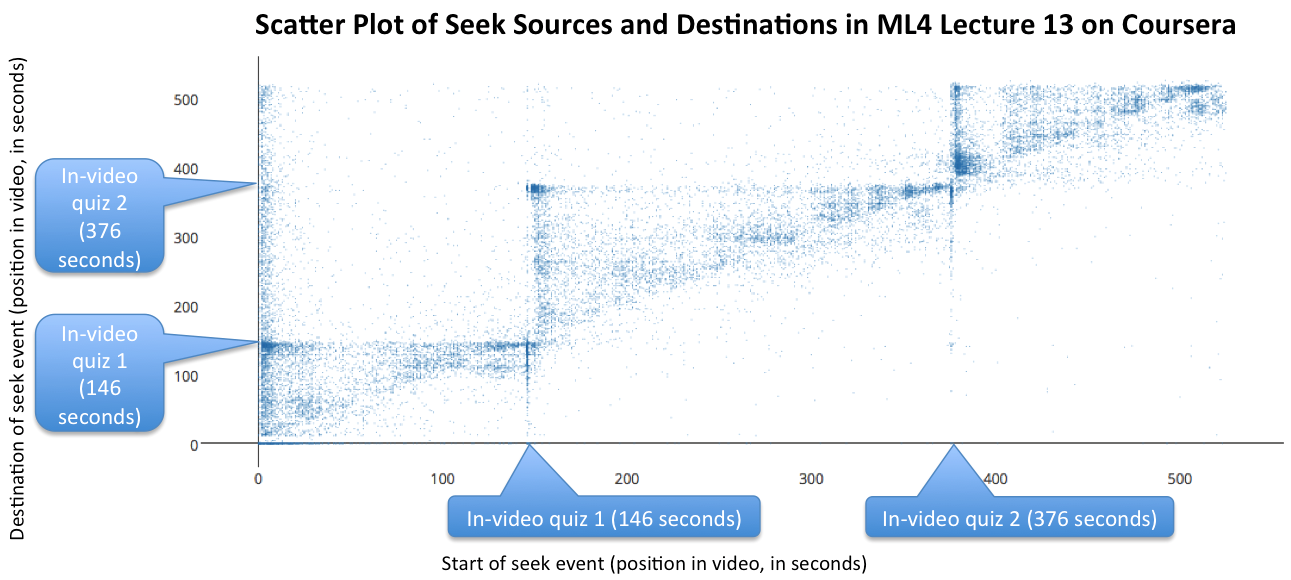
\includegraphics[width=\columnwidth]{seek-scatterplot}
\caption{Seeks sources and destinations in a lecture with 2 in-video quizzes. There are many seeks from the start of the video to the first in-video quiz (x=0, y=146), and between in-video quizzes (x=146, y=376).} % Backwards seeks tend to go from in-video quizzes (x=146 and x=376) to the preceding section.
\label{fig:seek-scatterplot}
\end{figure}

% In addition, we found that (less than 1/6 of users ever re-opened lecture videos), and that tended to 

% During our analysis of viewing logs for the Machine Learning course on Coursera, we observed that users' navigation behavior is heavily influenced by in-video quizzes. Users commonly seek to in-video quizzes, as shown in \autoref{seek-destinations}. Users seek to the in-video quiz primarily from the section of the video that immediately precedes it, as shown in \autoref{seek-scatterplot}. Some users even seem to follow a . Hence, we wished to make these questions. %Because users often seek forward to the in-video quiz that immediately follows the section, and back to the video from the quiz [Fig3], we thought they would benefit from being able to preview the upcoming quiz while viewing the lecture, without needing to seek to the in-video quiz.

% Online lectures focus heavily on viewing video content. However, a phenomenon known as the \emph{testing effect} shows that actively quizzing learners on the content is more effective for retention than simply having them passively watch videos \cite{testingeffect}. Platforms such as Coursera have in-video quizzes which bring the benefits of testing into the video context by asking the user a multiple-choice question at key points in the video about the content that they have just watched. However, in-video quizzes are still given relatively little focus: they are shown only after the relevant segment has been viewed, are often skipped by users.

Our system, Quiz-driven Video Cramming (QuizCram), uses quizzes to help users navigate the course and direct their review process. It includes the following features:

\begin{compactitem}
\item Our interface shows the question while the user watches the video, so it serves as an advance organizer to prime them towards the key concepts they should focus on %while watching the video.
% \item Our system provides useful feedback in response to an incorrect answer, encourages the user to review the relevant portion of the video, and enforces that users can answer the question on their own before advancing them to the next portion of the video.
% \item To encourage people to review videos, our system keeps track of which video portions users need to review (using a score based on question scores on associated segments, percentage of the segment reviewed, and recency of reviewing), and gives them suggestions of questions and video portions to review once they have watched all the video segments.
\item To encourage people to review videos, our system keeps track of which video portions users need to review, and gives users suggestions of questions and video portions to review %once they have watched all the video segments.
\item We allow questions to be added more easily to videos, by allowing questions depend on video segments other than just the immediately preceding one. This allows for there to potentially be a higher density of questions in the QuizCram format.
\end{compactitem}

We used a within-subjects study to compare QuizCram to the in-video quiz format. We found:

% To evaluate the effectiveness of QuizCram for helping users study, we used a within-subjects study design comparing it to an in-video quiz format. Our contributions are:

\begin{compactitem}
% \item QuizCram, a format for viewing lectures in an interactive, question-centric manner, that can be automatically generated from existing videos with in-video quizzes.
\item Answers to in-video questions are remembered significantly better when users are using QuizCram
\item Users practice answering and reviewing questions more often when using QuizCram
\item We can improve the recall of particular facts from the video by adding extra questions in QuizCram.
% \item Users are satisfied with QuizCram, and find the interface features for answering questions and reviewing videos to be helpful.
\end{compactitem}

% =============================================================================
\section{Related Work}
% =============================================================================
We designed QuizCram's features based on the following findings from the education literature:%, which are also exploited by many other systems.

\subsection{Testing and Pre-Testing Effects}

The \emph{testing effect} shows that repeated testing combined with fast, informative feedback helps students remember material \cite{testingeffect}. QuizCram's emphasis on answering and reviewing questions is designed to exploit this effect.

% The testing effect finds that repeated testing combined with fast, informative feedback helps students remember material \cite{testingeffect}. In-video quiz systems are based on this principle: by testing the user on the video contents that were just viewed, they help students remember the material \cite{guidingquestions}. QuizCram's question-directed studying approach is also designed to exploit the testing effect.

The \emph{pre-testing effect} shows that asking users to try answering a question before they actually study the material enhances long-term retention \cite{pretesting}. QuizCram exploits the pre-testing effect by allowing users to preview the question before watching the associated video.

\subsection{Advance Organizers: Video Transcript Summaries}

Advance organizers are information presented prior to learning, that help the learner process the material that is about to be presented  \cite{advanceorganizers}. Video Digests is a system that creates such summaries about videos, and uses them as an advance organizer and navigational guide for video lectures \cite{videodigests}. QuizCram similarly breaks videos into segments associated with an advance organizer, but we use existing in-video questions to summarize the clips.

% Advance organizers are information presented prior to learning, that help the learner process the material that is about to be presented  \cite{advanceorganizers}. An example of an advance organizer for lecture video content would a summary of the video content that is to be watched. Video Digests is a system that creates such summaries about videos, and uses them as an advance organizer and navigational guide for video lectures \cite{videodigests}. Our system follows a similar strategy of breaking the video into segments associated with an advance organizer, but we instead use a question as an advance organizer that summarizes the clip to the user before they start watching it.

\subsection{Spaced repetition: Flashcards}

% Spaced repetition is a technique designed to help learners retain information by having them review  items at regular intervals \cite{karpicke2011spaced}. A class of applications that exploit this are flashcards, where information is split into independent chunks that are scheduled for review based on factors such as mastery and recency of review. % Flashcards can also have associated multimedia, such as video clips.

Spaced repetition is a technique used by flashcards to help learners retain information by having them review items at regular intervals \cite{karpicke2011spaced}. Similar to flashcards, our system also schedules questions for review based on our model of the user's mastery and recency of review. % A key difference is that lecture videos build on each other, so we must schedule earlier videos first.

% Spaced repetition is a technique designed to help learners retain information by having them review  items at regular intervals \cite{karpicke2011spaced}. A class of applications that exploit this are flashcards, where information is split into independent chunks that are scheduled for review based on factors such as mastery and recency of review. Similar to flashcards, our system also schedules items for review according to mastery and recency of review.

% Similar to flashcards, our system also schedules items for review according to mastery and recency of review. One key difference is that lecture videos build on each other, so this is an additional constraint for scheduling: the user needs to have covered the previous videos. % Another key difference is the cost of review: a user memorizing vocabulary using flashcards only needs to spend a few seconds on each flashcard, while answering a question or reviewing a video clip takes an order of magnitude more time. Hence, the user will make fewer review passes through the video content than they would with vocabulary flashcards.
% =============================================================================

% =============================================================================
%\begin{figure}
%\centering
%\includegraphics[width=1.0\columnwidth]{singlevideo-overview}
%\caption{The QuizCram interface, showing the current video. The focus question is on left, and the associated video is on the right. The progressbar highlights the relevant portion of the video in yellow. Already-watched segments of previous sections is in blue, already-watched segments of the current part are in green. Because we are currently watching a section we have already viewed, an option to skip to the unseen portion is shown.}
%\label{fig:figure1}
%\end{figure}

\section{System Design}

% QuizCram's interface shows users a question to review, with an associated video segment, as shown in \autoref{fig:figure3}. It also shows a scrollable timeline of previously answered questions and associated video segments below the current question. Questions are first scheduled in order, then once the user has made an initial pass, questions are selected for review algorithmically, based on historic correctness of responses, percentage of associated video that has been watched, and the recency of review. We also use the video progressbar to indicate the section of the video that is relevant to the current question, and portions of the video that the user has previously seen.

QuizCram's interface displays a question and associated video segment, as shown in \autoref{fig:figure3}. It also shows a timeline of previous questions below the current question. Once the user has made an initial pass through the questions, we suggest questions that they should review, based on past performance. We use the video progressbar to indicate the section of the video that is relevant to the current question, and portions that the user has previously seen. An existing course with in-video quizzes, such as MOOCs on Coursera, can be automatically transformed into the QuizCram format. 

\begin{figure}
\centering
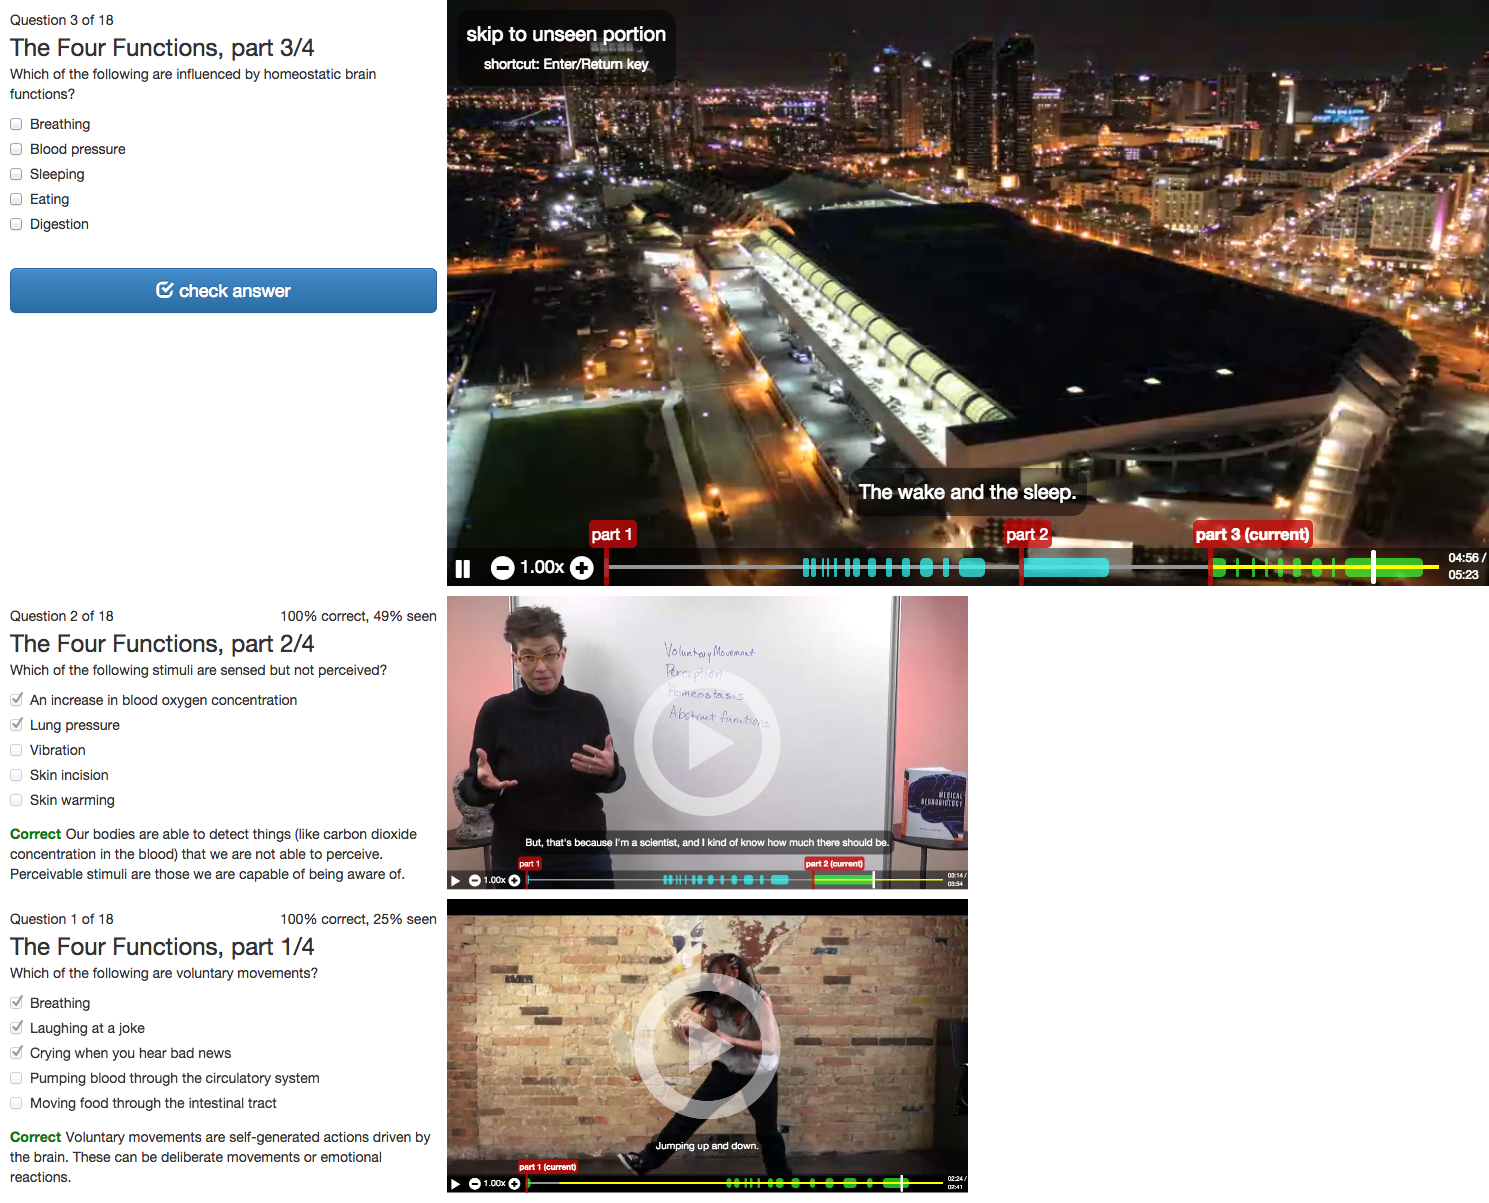
\includegraphics[width=1.0\columnwidth]{quizcram-and-timeline2}
\caption{The scrollable timeline, shown below the current question, displays the past videos and associated questions, to help users review parts they had trouble with.}
\label{fig:figure3}
\end{figure}

% An existing course with in-video quizzes, such as MOOCs on Coursera, can be automatically transformed into the QuizCram format. This results in each video segment having one associated question. However, unlike in-video quizzes, the QuizCram format can also have multiple questions associated with a single video segment.

% =============================================================================
\subsection{Question-Directed Video Viewing}
% =============================================================================
% For each section of the video in the course, we have one or more associated questions. We can get these question-video pairs automatically from existing videos with in-video quizzes, by associating the in-video quiz section with the immediately preceding video segment. For video segments that did not have an associated in-video quiz, we can either automatically insert a generic ``How well did you understand this video'' question, or manually write a new question.

Each section of the video in the course is displayed with an associated question, as shown in \autoref{fig:figure3}. The question is designed to help users decide whether they should watch the video. If the user knows the answer, they can answer the question and move to the next section. For users who do not  know the answer, reading the question summarizes the key points they will see in the video.

% Unlike in-video quizzes, which users are freely able to skip over, in QuizCram the user must correctly answer the question before they can move on to the next question and associated video segment. This is designed to ensure that users learn the material before advancing onwards, as opposed to simply passively watching the videos without testing themselves.

% Forcing users to answer the question may lead to frustration if the user is unable to determine the correct answer even after watching the video. Hence, whenever the user answers the question incorrectly, we provide them with immediate, informative feedback by showing the answers and providing an explanation, as opposed to the model used by Coursera where it states that the answer is incorrect, and only shows the explanation and correct answer after 3 tries. We made this design choice based on literature that finds that specific feedback that explains the correct answer to learners is more helpful and motivates them more than simply stating that their answer is incorrect \cite{formativefeedback}.

%\begin{figure}
%\centering
%\includegraphics[width=1.0\columnwidth]{incorrect-responses2}
%\caption{In response to an incorrect response, the user is asked to view an additional 10\% of the video, the answer options are shuffled, and the user needs to re-answer the question correctly before moving on.}
%\label{fig:figure2}
%\end{figure}

% Of course, immediately showing the answer in response to an incorrect answer leads to the risk that learners may choose to immediately reveal the answer without attempting to answer the question themselves. To discourage such behavior, even though we show the user the answer and explanation in response to an incorrect response, we do not advance them automatically. Rather, we shuffle the answer options and require them to view an additional 10\% of the video, which is roughly 20 seconds, before attempting to answer it again, as shown in \autoref{fig:figure2}. We do not enforce the 10\% viewing requirement if the user has already watched over 75\% of the video. This viewing task encourages users to view unseen portions of the video, incentivizes users to answer questions correctly, and ensures they aren't simply storing the answers in short-term memory and reproducing them. Requiring users to view the video and then retesting them after an incorrect response creates an additional retrieval opportunity, which should improve retention of the material \cite{testingeffect}.

% While shuffling the answers and requiring video watching in response to an incorrect response discourages users from simply submitting the incorrect response and memorizing the answers, it does not entirely eliminate the risk. We can further discourage memorization of answers by having multiple questions for each video segment, which we alternate between. For example, in a algebra context we could simply ask the question again with different variable values whenever the user responds incorrectly. However, we did not use this option in our user studies since it would require us to write additional questions.

\subsection{Timeline of Previous Questions and Videos}

The \emph{timeline} feature is designed to encourage review by making it easy to refer back to previously answered questions and video segments. Whenever a question is correctly answered, we insert the next question and associated video segment at the top of the interface, and push the existing questions down. This results in a scrollable visual history of the previously answered questions, as shown in \autoref{fig:figure3}. The timeline displays the question, its answer, and a miniaturized version of the video which can be clicked to enlarge it to full size and play it. The miniaturized video displays the frame the user left off at, so it serves both as a visual summary, and also allows users to easily resume watching previous videos.% where they left off.

By organizing the list of previous video segments according to the associated question that users answered, this allows users to scan video segments with a more salient summary than just the title. Question-based video navigation also allows users to search at a higher granularity, as questions refer to a specific subsection of the video, while the title refers only to the entire video contents.

% Although QuizCram focuses the user's attention towards the current question and associated video segment, we also wish to make it easy to refer back to the previously answered questions and video segments. Whenever a question is correctly answered, we insert the next question and associated video segment at the top of the interface, and push the existing questions down. This results in a scrollable visual history of the previously answered questions and videos which we call the \emph{timeline}, shown in \autoref{fig:figure3}. The timeline displays the question and its answer and a miniaturized version of the video which can be clicked to enlarge it to full size and play it. The miniaturized video displays the frame the user left off at, so it serves both as a visual summary, and also allows users to easily resume viewing progress of previous videos. % We also show the historic correctness of the user's answers to that question, and percentage of the video they have watched, to help users identify questions they had trouble with and videos they did not fully watch.

% The timeline gives users the option to use a more traditional, self-directed reviewing strategy, in contrast to the flashcard-style reviewing that our question scheduling algorithm encourages. By organizing the list of previous video segments according to the associated question that users answered, this allows users to scan video segments with a more salient summary than just the title. Question-based video navigation also allows users to search at a higher granularity, as questions refer to a specific subsection of the video, while the title refers only to the entire video contents. % Furthermore, re-reading the previously answered questions helps trigger the users' memory of the associated clip, giving learners another retrieval opportunity to solidify their memory of the video contents.

\subsection{Scheduling Questions and Video Sections for Review}

% We want users to spend their study time focusing on material that they have not yet mastered. Hence, we assign each question a \emph{mastery score}, which represents how well the user currently knows the material, and show users the questions for which they have low mastery score. The question's mastery score is based on the following 3 factors:

We want users to spend their study time focusing on material that they have not yet mastered. Hence, we assign each question a \emph{mastery score}, which represents how well the user currently knows the material, and show users the questions for which they have low mastery score. The mastery score is a weighted sum based on the user's past performance on the question, the fraction of the associated video segment they have watched, and the recency of review.

Once the user has seen all the questions in the unit, QuizCram encourages them to review questions and sections for which they have low mastery scores, by showing them at the top of the video timeline.

% \begin{itemize}
% \item \emph{Past performance on question}: This element of the score encourages users to review questions they answered incorrectly. Each time a user tries answering the question, we give them a score between 0 to 1 based on the percent of checkboxes they correctly checked (the questions used in our study were all multiple-check questions). We then do a weighted-mean of all historic scores, with each newer score assigned 2 times more weight than the previous score (so more recent performance is weighted more heavily). For those video segments that have no associated question, we obtain this score by asking users to rate ``How well did you understand this video?''. If the user has never answered the question before, this has a default score of 0.
% \item \emph{Fraction of associated video segment watched}: This element of the score encourages users to view video segments they have not seen. For each section of video, we keep track of whether the user has ever watched it. This score is the number of seconds watched in the question's video segment, divided by the total length of that video segment.
% \item \emph{Recency of review}:  This element of the score encourages spaced repetition for the questions. It also ensures that users are not shown the same questions repeatedly, which would make users bored. It is equal to 1 / number of questions elapsed since this question was last seen by the user. If the question has never been seen, this has a default score of 0.
% \end{itemize}

% The mastery score is a weighted sum of these factors, where question correctness is 4/7 of the score, fraction of the video watched is 2/7 of the score, and recency of review is 1/7 of the score. We assign question correctness the highest priority because users should all be able to answer the questions correctly, but some users may choose to not watch portions of video they consider irrelevant or already know.

% Sorting by the mastery score alone does not enforce that users have met the prerequisites for understanding the video and answering the question, before we show them the video and question. Unlike flashcards, lecture videos are meant to be watched in order and build on each other, so each video segment has a set of prerequisite videos which need to be watched before students can understand them. In our implementation, we enforce prerequisites by requiring that the user has correctly answered the questions for preceding video segments, before we show them the next video segment and associated question.

% Sorting questions by mastery score and enforcing the prerequisites effectively results in users first being shown questions that work them through the videos in the order the course covers them, then asking them to review the questions they got low scores for and videos did not finish watching.

% \subsection{Directing Attention to Parts of Video Relevant to Question}

% Standard in-video quiz viewers show the entire video at once. However, QuizCram shows only the part of the video relevant to answering the question, specifically, the start of the video up until the point where the question would be located (in an in-video context). We additionally highlight in yellow the section of the progressbar where question answer is located. This is designed to focus the user's attention to the portion of the video that will help them answer the question.

%\begin{figure*}
%\centering
%\includegraphics[width=2.0\columnwidth]{highlighting-relevant-portions}
%\caption{We highlight portions of the video that are relevant to the current question. This gives additional flexibility in question writing and placement: if the question depends on a portion of the video from a previous part, as in this example, we can highlight that section in the video progressbar to indicate that it is relevant to the current question}
%\label{fig:figure4}
%\end{figure*}

% QuizCram highlights on the progressbar the portion of the video that is relevant to answering the current question. For questions generated from in-video quizzes, we highlight the segment of the video that immediately preceded the in-video quiz, as shown in \autoref{fig:figure1}. However, because we can highlight any preceding portion of the video to indicate that it is relevant to the current question, this give us flexibility in question writing and placement: we can place questions where they would fit most naturally. This also enables us to have multiple questions that cover a single segment of video, without confusing users about where the answers to the questions are located.

% For questions generated from in-video quizzes, we highlight the segment of the video that immediately precededs the in-video quiz to indicate that it is where the answer is found, as shown in \autoref{fig:figure1}. However, because we can highlight any preceding portion of the video to indicate that it is relevant to the current question, this also allows us to have more flexibility in question writing and placement: we can place questions where they would fit most naturally, rather than immediately following the section where the answer is covered. This also enables us to have multiple questions that cover a single segment of video, without confusing users about where the answers to the questions are located.

\subsection{Directing Attention to Unseen Parts of Videos}

To help users review videos, QuizCram keeps track of which parts have been watched. It highlights on the progressbar the portions that have already been seen. If the user is viewing a section they have already watched, they can skip to the unseen portion by clicking a button. % Similar techniques for visualizing the user's video viewing history have been presented in the literature \cite{socialnavigation} \cite{lecturescape}, though our system adds the novel feature of allowing users to skip to the next unseen portion.

%\begin{figure}
%\centering
%\includegraphics[width=1.0\columnwidth]{invideo-interface}
%\caption{The in-video quiz format that served as our baseline. Locations of quizzes are indicated in red on the progressbar.}
%\label{fig:figure5}
%\end{figure}

% =============================================================================
\section{Evaluation}
% =============================================================================
Our user study was an within-subjects study that compared users' studying behavior with QuizCram to an in-video quiz interface that mimcs the format used on Coursera. We used the videos, in-video quizzes, and unit exam from the Neurobiology course on Coursera. We wished to answer the questions:

\begin{compactitem}
\item Does QuizCram help users better remember answers to the original in-video questions?
\item Does QuizCram help users score higher on exams?
\item Can we improve recall of particular facts from the video by adding extra questions with QuizCram?
\item Do users find QuizCram helpful for studying videos?
%\item How do users use QuizCram?
%\item Do users using QuizCram answer questions more?
%\item Do users using QuizCram re-answer questions more?
\end{compactitem}

%\subsection{Study Design}

%The study was a within-subjects design, where each learner used QuizCram and an in-video quiz viewer interface to study a set of videos. They were asked to provide qualitative feedback immediately after viewing, and were tested on the material they studied a day later.

\subsection{Participants}

We recruited 18  students by posting on university mailing lists. 12 were female, 6 male. Their average age was 21.7 ($\sigma$=4.91, min=18, max=37). All had native-level English proficiency. None had prior exposure to neuroscience.  They received \$60 for participating. %in the 2-hour online study. % 9 participants reported having previous experience with MOOCs, and of these 6 had experience with Coursera.

\subsection{Materials}

% The course materials -- videos, in-video quizzes, and unit exams --- were the first and second halves of Unit 1 of an existing Neurobiology course on Coursera. We generated the initial QuizCram materials directly from the course. However, because we felt the question-to-video ratio in the original videos (9 questions for each 25-minute segment) was lower than what would be optimal for QuizCram, and because we wished to see the effects of inserting additional questions on recall of associated facts, we wrote additional questions for the QuizCram condition to double the total number of questions.

% We doubled the number of questions shown in the QuizCram condition by adding additional questions in the same style and format as the original multiple-checkbox in-video questions. We chose our questions carefully such that the answers were clearly stated in the video, but they would not ask the same facts that were tested on the unit exam or original in-video questions.

The videos, in-video quizzes, and unit exams were from Unit 1 of the Neurobiology course on Coursera. There were 9 questions and 5 videos for each 25-minute segment. We generated the initial QuizCram materials directly from the course. To see whether we could improve the recall of particular facts by adding questions, we added extra questions to the QuizCram condition to double the total number of questions. The extra questions were in the same multiple-checkbox format as the original questions. We made sure that they did not ask the same facts as the unit exam or in-video questions.

We also wrote a set of free-response questions, one corresponding to each of the extra multiple-checkbox questions. We used these free-response questions to test whether users had learned the material tested by in-video questions well enough to recall it.

% We also wrote a set of free-response questions, one corresponding to each of our extra multiple-checkbox questions. For example, the question ``Which of the following are true of astrocytes?'' followed by 3 true options and 2 false options would be transformed into the free-response question ``List 3 facts about astrocytes''. We used these free-response questions to test whether users had actually learned the material tested by our new questions well enough to recall it, as opposed to simply learning to recognize the answers when presented in multiple-checkbox format.

\subsection{Procedure}

% The study was conducted online over 2 days, with a 90-minute study session on the first day, and a 30-minute test session on the second day. % Before users started the study, we informed them that they would be given 2 sets of videos, they should study them for 40 minutes apiece, and they would be given an exam the next day. % We did not tell them about the content of the exams.

The study was conducted online over 2 days. On day 1, users were given 40 minutes to study the first section with the first tool. Then, they used the other tool to study the second section for 40 minutes, and filled out a survey. On day 2, users took the following exams:

% On the first day, users used one tool to watch the first half of Unit 1 (5 videos of length 23 minutes total). They were told after 40 minutes to fill out a survey about the tool. Then, they used the other tool to watch the second half of Unit 1 (5 videos of length 25 minutes total), and filled out the survey after 40 minutes of watching.

\begin{compactenum}
\item Extra free-response questions %, both halves
\item Original in-video questions from Coursera%, both halves
\item Original unit exam from Coursera%, both halves
\item Extra multiple-checkbox questions %, both halves
\end{compactenum}

%Parts 2-4 of the exam were automatically graded, giving each question a score equal to the fraction of checkboxes correctly checked. % The free-response questions, which were of the general form ``List N examples of X'' or ``State N facts about X'', were graded by first marking each example provided by students as correct or incorrect. % Examples and facts did not need to be the same ones provided in the video -- so long as they were appropriate to the question and correct, they were marked as correct.
% Then, we scored each response via the formula:
% Parts 2-4 of the exam were automatically graded, assigning scores equal to the fraction of checkboxes correctly checked.
% The free-response questions, which were of the form ``List N examples of X'' or ``List N facts about X'', were scored as:
%Parts 2-4 of the exam were automatically graded, assigning scores equal to the fraction of checkboxes correctly checked. The free-response questions were graded by an independent grader.
Parts 2-4 were automatically graded. Free-response questions were graded by an independent grader.

%\vspace{-4mm}

%\[ \frac{\# correct\ examples\ given}{Maximum(\# examples\ requested,\ \# examples\ given)} \]

% Thus, if a question requests 2 examples, giving 1 correct example gets a score of 1/2, giving 2 correct examples and 1 incorrect example gets a score of 2/3, etc. The overall score for the free-response exam was the mean of these scores.

% We chose this design of having users watch both sets of videos before taking any exams, as opposed to having them take an exam after they finished studying each section, because this way the user does not know that the exam includes the in-video questions, so this does not influence their study behavior. In previous versions of this study we had observed that if users know they will be tested on in-video questions, either by taking the exam or if we told them, they will explicitly study them and will have near-perfect scores on those parts of the exam, but not the rest of the exam. We instead chose our current study design so that we can observe the tool's effect on in-video question retention in natural study contexts where the user knows nothing about the exam.

\subsection{Exam Results}

Exam results are shown in \autoref{fig:exam-results}.  Users using QuizCram performed significantly better at answering the original in-video questions. We attribute this difference to the increased prominence of questions in the QuizCram interface. They also performed better at the extra questions, both multiple-choice and free-response. This suggests that we can use added questions in QuizCram to improve retention of particular facts from the video.

\begin{figure}
\centering
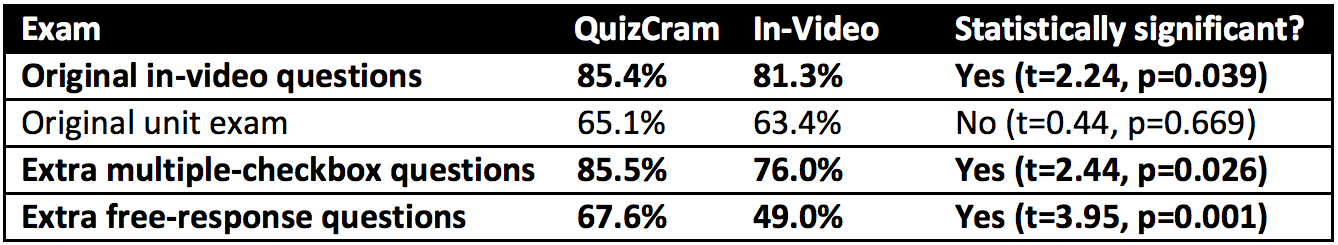
\includegraphics[width=1.0\columnwidth]{exam-results}
\caption{Average exam scores for each condition}
\label{fig:exam-results}
\end{figure}

% \subsubsection{Exam Results for Original In-Video Questions}

% Users were better able to answer the original in-video questions when using QuizCram. They averaged 85.4\% with QuizCram, compared to 81.3\% with the in-video quiz format. This difference was statistically significant (t=2.24, p=0.0391). % The average scores between in-video questions for the two halves were similar -- 84.5\% average for part 1, 82.2\% average for part 2, with no significant difference (t=0.55, p=0.589).

% Thus, even though the users encountered the original in-video questions in both conditions, the QuizCram format caused them to remember the answers better. We attribute this difference to the increased prominence of questions in the QuizCram interface, and requirement that questions be answered correctly by the users before proceeding onwards.

% \subsubsection{Exam Results for Unit Quiz}

% Unit exam scores were similar when using QuizCram compared to the in-video condition. Average scores on the portion of questions covered by QuizCram was 65.1\%, while scores for the questions from the portion viewed using the in-video interface was 63.4\%. This difference was not significant (t=0.44, p=0.669). % Users performed slightly better on the questions from the second half of the unit exam: the average score was 59.2\% for questions covering the first half of the videos, and 69.3\% for questions covering the second half of videos (t=-1.98, p=0.064).

% This result is not unexpected, given that the unit quiz questions covered different concepts than those the in-video quizzes focused on, even though they were both covered in the videos. Our inserted questions likewise did not overlap with the unit quiz questions, to avoid giving QuizCram users an unfair advantage on the unit quiz. This suggests that even though QuizCram's question-centric viewing approach helps learners learn the concepts that are tested in the questions, it does not appear to help them with portions of the video that are not tested.

% \subsubsection{Exam Results for Extra and Free-Response Questions}

% Users were better able to answer the extra questions we inserted in the QuizCram condition when viewing the section with QuizCram. They averaged 85.5\% with QuizCram, compared to 76.0\% with the in-video interface. This difference was statistically significant (t=2.44, p=0.0260). % This is expected: users had previously seen these questions if they were using QuizCram, but they were not shown to users in the in-video quiz condition.

% Users were also better able to answer the free-response questions when using QuizCram. They averaged 67.6\% correctness with QuizCram, compared to 49.0\% correctness with the in-video quiz format. A t-test showed this difference was statistically significant (t=3.95, p=0.0010). % The average scores between the two halves were similar -- 59.4\% average for part 1, 57.1\% average for part 2, with no significant difference (t=0.35, p=0.731).

% Although the users who used QuizCram had never seen the free-response questions before, the questions covered similar material to the extra multiple-checkbox questions we had inserted for the QuizCram format, except in free-response format. This suggests that when using QuizCram, users are not simply learning how to recognize the correct answers for questions, but are also learning to recall them. It also suggests that if there is a particular piece of information that the instructor would like the class to be able to recall, inserting it as an additional question into the QuizCram system is one possible way to accomplish this goal.

\subsection{Survey Results}

When asked to rate their overall satisfaction with the tool a scale of 1 to 7, the average was 5.28 for QuizCram, and 5.17 for the in-video quiz format.  61\% indicated they would prefer using QuizCram if they wanted to remember material long-term or were preparing for an exam.

Users liked QuizCram's question-based segmentation of videos, and thought it was helpful for reviewing questions. However, some users thought that the emphasis on questions distracted them from watching the video.

\subsection{Analysis of Viewing Logs}

% Users practiced answering questions more times when using QuizCram, as shown in \autoref{fig:event-logs}. Users also reviewed questions more often when using QuizCram. This increase in practice and reviewing helps explain the increased scores on the in-video questions during the exams.

To compare how users were using the two systems, we logged usage data for each tool, as shown in \autoref{fig:event-logs}. We found that users practiced answering questions more times when using QuizCram. Users also reviewed questions more often when using QuizCram. This increase in practice and reviewing helps explain the increased scores on the in-video questions during the exams. % when using QuizCram.

% To compare how users were using the two systems, we logged the number times users answered questions or seeked with each tool, as shown in \autoref{fig:event-logs}. We found that users practiced answering questions more times when using QuizCram. Users also reviewed questions more often when using QuizCram (we defined ``reviewing'' as re-answering a question at least a minute after they first answered it). This increase in practice and reviewing helps explain the increased scores on the in-video questions during the exams.

Users seeked less on average when using QuizCram, which may be because they did not have to seek to and from in-video quizzes. However, this difference was not statistically significant.

\begin{figure}
\centering
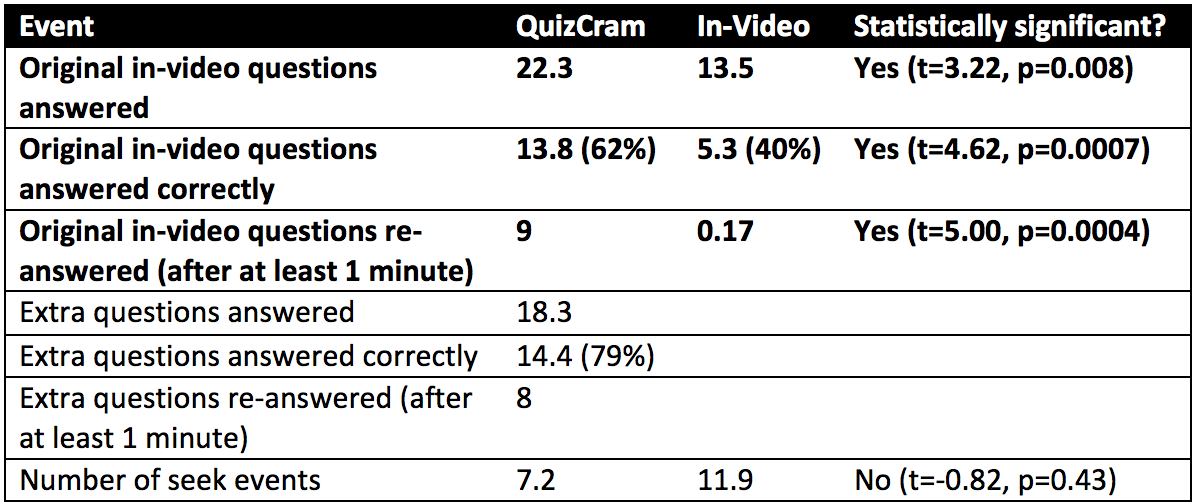
\includegraphics[width=1.0\columnwidth]{event-logs}
\caption{Average number of events per user in each condition}
\label{fig:event-logs}
\end{figure}

% Users reported their preferences as follows:
%After users had used both tools, they responded with their preferences as follows:

%\begin{itemize}
%\item In response to ``Which tool would you rather use for studying?'', 9 (50\%) preferred QuizCram.
%\item In response to ``Which tool would you rather use for studying if you were preparing for an exam and were short on time?'', 11 (61\%) preferred QuizCram.
%\item In response to ``Which tool would you rather use for studying if wanted to remember the material long-term?'', 11 (61\%) preferred QuizCram.
%\end{itemize}

% When asked to rate ``Overall, I am satisfied with using this video viewing tool'' on a scale of 1 (strongly disagree) to 7 (strongly agree), the average was 5.28 for QuizCram, and 5.17 for the in-video quiz format. % Hence, users appeared to be satisfied with both formats.

% When asked to list what they liked about each format, users said that they liked how QuizCram displayed the question alongside the video, they liked the question-based segmentation of the video, and mentioned that it was helpful for reviewing questions they had answered incorrectly:

%\emph{It was a good fit for me to read and answer questions, while the video was playing. I appreciate how wrong answers were handled with information leading to correct answers.}

% Users generally liked QuizCram's question-focused format:

%  \emph{I liked that it picked out the key information I should retain by asking me questions. It helped me decide what to focus on as I watched the video. The chunks were very manageable as well. I liked how it was broken up.}

%\emph{It was easy to review the questions and quiz myself multiple times, and ultimately, the repetition aided my understanding of the material.}

% \emph{I liked how once I was done, and I still had time in my 40 min, then I could go back to videos where I'd gotten questions wrong the first time on the quiz and review. I liked that sometimes, if I got the questions wrong, then the answers were switched around forcing me to read the answers again.} 
%Also, having the questions from the beginning made me focus more on the answers to the questions than listening to the whole lesson material. I made a game with myself out of seeing when I thought I knew enough to answer the questions (without listening to the whole video). Then I'd listen to the whole video afterward. 

% When asked to list what they disliked about each format, the primary complaints about QuizCram were that showing the question at all times distracted them from the video, and that it was not possible to skip ahead without answering questions:

% \emph{I felt compelled to answer the questions correctly instead of watching the video to absorb the information. Perhaps only being able to preview the question before watching the video and then having access to answer it afterwards would help.}

%\subsection{Usage Patterns}

%To see how users were interacting with the system, we logged interaction data during our study. We were particularly interested in observing how users used the system as a review tool. 


% =============================================================================
%\section{Discussion}
% =============================================================================
% The design goal behind QuizCram is to increase users' focus on questions, utilizing questions as a means to navigate and review the video material. Our user study finds that QuizCram indeed does increase focus on questions -- when the questions presented during viewing were tested again a day later, users using QuizCram performed better at answering the questions than users who encountered the questions as in-video quizzes. Users' qualitative feedback likewise indicates that they felt questions were an important part of the system. Users were were divided in preferences between the QuizCram format and the standard in-video quiz format. Some users liked the question-directed viewing format and thought it was more engaging, though others thought the questions were distracting.

%The design goal behind QuizCram is to increase users' focus on questions, utilizing questions as a means to navigate and review the video material. QuizCram keeps track of users' historic performance on questions and video progress, and makes suggestions for questions and associated segments of video to review. Thus, it relieves the user of the mental burden of needing to keep track of their study progress and determine what they need to review.

% The design goal behind QuizCram is to increase users' focus on questions, utilizing questions as a means to navigate and review the video material. Our user study focused on a short-term study task, modeling an exam-cramming scenario. In reality, however, we want to remember the contents of entire courses rather than single units, and need to study it across the period of months rather than hours. 

%When reviewing lectures with traditional interfaces, the user needs to keep track of what they remember and what they need to review. This may be an easy task if they are reviewing only an hour of video. However, when studying entire courses over the course of a month, a user can easily lose track of what their study progress was. Instead, QuizCram keeps track of users' historic performance on questions and video progress, and makes suggestions for questions and associated segments of video to review. Thus, it relieves the user of the mental burden of needing to keep track of their study progress and determine what they need to review.

%Another interesting finding was that with QuizCram, we were able to increase the number of questions associated with a video segment without adversely effecting the user experience or exam performance. In fact, we find that users remember the material covered by these additional questions well enough to answer them in free-response format. This paves a way for further increasing the amount of testing that occurs within video content.

%Current online courses have external problem sets and quizzes outside of the ones in videos, because they cannot test the content in sufficient depth using in-video quizzes. However, if we consider the engagement patterns of users with MOOCs, the majority of users are interacting only with the videos and never doing the problem sets or quizzes \cite{anderson2014engaging}. Thus, moving more of the course content out of external quizzes and making the video more interactive and question-oriented provides a way to benefit these viewers' learning by testing their knowledge, without removing them from the scaffolding of videos. By gradually moving along this trajectory of making videos more question-focused and recommending review material to users, online courses of the future could entirely eliminate their need for external problem sets and quizzes, and transform into video and question-based intelligent tutoring systems.

% The design goal behind QuizCram is to increase users' focus on questions, utilizing questions as a means to navigate and review the video material. Our user study finds that QuizCram indeed does increase focus on questions -- when the questions presented during viewing were tested again a day later, users using QuizCram performed better at answering the questions than users who encountered the questions as in-video quizzes. Users' qualitative feedback likewise indicates that they felt questions were an important part of the system. Users were were divided in preferences between the QuizCram format and the standard in-video quiz format currently predominant in MOOCs. Some users liked the question-directed viewing format and thought it was more engaging, though others thought the questions were distracting.

% We were pleased to find that encountering questions in multiple-checkbox form in QuizCram caused users to remember the tested content sufficiently well that they were able to answer it in free-response format a day later. Likewise, we found that it is possible to double the question-to-video ratio in the context of QuizCram. This 

% =============================================================================
\section{Conclusion}
% =============================================================================
We have presented QuizCram, a system that direct users' video viewing using questions. QuizCram aims to:

\begin{compactenum}
\item Encourage users to answer and review questions while they watch videos
\item Enable users to easily follow question-driven video navigation strategies (which we currently observe some users already using on Coursera)
\end{compactenum}

QuizCram breaks the video into segments associated with questions, and always shows a focus question alongside the video. The focus question serves as an advance organizer that directs the user's attention towards the key points in the video. QuizCram also encourages reviewing based on questions: it displays a timeline of questions previously answered and their associated videos. It keeps track of users' progress through questions and videos, and suggests questions for users to review. Courses in the QuizCram format can be automatically generated from existing video content with in-video quizzes, though it also has the flexibility to accommodate additional questions.

% Based on our observations that in-video quizzes play an important role in video navigation, we designed QuizCram, a system that uses questions to direct users' viewing of the material. It allows users to preview the question for the sections, and provides a timeline of questions and suggestions to encourage reviewing.

Our user study finds that QuizCram increases focus on questions -- when the questions presented during viewing were tested again a day later, users using QuizCram remembered them better than if they were presented as in-video quizzes. Users practiced answering and reviewing questions more often when using QuizCram. We also found that increasing the amount of questions presented with QuizCram results in users remembering the material tested by the additional questions better, even when answering based on recall not recognition.

Current online courses have external problem sets and exams, to test content in more depth than is covered by in-video quizzes. However, the majority of users on MOOCs are interacting only with the videos and never doing the problem sets or exams \cite{anderson2014engaging}. Thus, moving more of the course content out of external problem sets and making the video more interactive and question-oriented provides a way to benefit these viewers, without removing them from the scaffolding of videos. We believe that QuizCram is a logical step from in-video quizzes towards more interactive, question-driven video viewers. % By gradually moving along this trajectory of making videos more question-focused and recommending review material to users, online courses of the future could entirely eliminate their need for external problem sets and quizzes, and transform into video and question-based intelligent tutoring systems.

% Users' qualitative feedback indicates that they felt questions were an important part of the system. Users were divided in preferences between the QuizCram format and the standard in-video quiz format currently predominant in MOOCs. Some users liked the question-directed viewing format and thought it was more engaging, though others thought that displaying the questions were distracting. We believe the QuizCram format is a logical step from the in-video quiz format towards more interactive, question-focused intelligent video viewing platforms.

% The video is divided into segments associated with a question, and there is always  . Once uses. Courses in the QuizCram format can be generated from existing videos with in-video quizzes. However, the format is also flexible enough to accomodate the insertion of 

%\balance

\bibliographystyle{acm-sigchi}
\bibliography{quizcram}
\end{document}

\end{document}